\documentclass[conference]{IEEEtran}

\IEEEoverridecommandlockouts
% The preceding line is only needed to identify funding in the first footnote. If that is unneeded, please comment it out.
\usepackage{cite}
\usepackage{amsmath,amssymb,amsfonts}
\usepackage{algorithmic}
\usepackage{graphicx}
\usepackage{textcomp}
\usepackage{xcolor}
\usepackage[utf8]{inputenc}
\usepackage[hidelinks]{hyperref}
\usepackage[normalem]{ulem}  % for \ulem
\usepackage{xspace}

\def\BibTeX{{\rm B\kern-.05em{\sc i\kern-.025em b}\kern-.08em
    T\kern-.1667em\lower.7ex\hbox{E}\kern-.125emX}}
\newcommand{\todo}[1]{\colorlet{saved}{.}\color{blue}#1\color{saved}}
\newcommand{\TG}[1]{\colorlet{saved}{.}\color{orange}From Tristan: #1\color{saved}}
\newcommand{\BJ}[1]{\noindent{\color{cyan}[\textsc{BJ:} #1]}\xspace}
\newcommand{\english}[1]{\uwave{#1}}  % English needs to be revised: it's either unclear or incorrect
\begin{document}

\title{High-Resolution Road Vehicle Collision Prediction for the City of Montreal}
\author{\IEEEauthorblockN{Antoine Hébert$^*$, Timothée Guédon$^*$,
Tristan Glatard, Brigitte Jaumard}
Department of Computer Science and Software Engineering \\
Concordia University, Montréal, Québec, Canada\\
$^*$ These authors have contributed equally

}

\maketitle

\begin{abstract}

Road accidents are an important issue of our modern societies, responsible
for millions of deaths and injuries every year in the world. \BJ{???: mais pas a Montreal (comme indiqu\'e dans le titre), peut-etre plusieurs ann\'ees, ou sinon le cout pour SAAQ}
In this paper, we show how one can leverage open datasets of a city like
Montreal, Canada, to create accident prediction models, using state-of-the-art
big data analytics.
Such models could be used in the context of road accident prevention, but also
to identify key factors that can lead to a road accident, and consequently, help
elaborate new policies.

We tested various machine learning methods to deal with the severe class imbalance inherent
to accident prediction problems. In particular, we implemented the Balanced Random Forest algorithm, a variant
of the Random Forest machine learning algorithm, into the Scala and Python
APIs of Apache Spark \TG{Is the PR in?} \BJ{Not sure the details of scala/Python are needed in the abstract}.

Experimental results show that our learning model identifies as positives 13\% of the data
points with the highest risk of collision, which corresponds to 85\% of 
vehicle collisions.
In addition, we identify the most important predictors of vehicle collisions for the area of Montreal: the count of accidents on the same road segment during previous years, the temperature, the day of the year, the hour and the visibility.

\end{abstract}

\begin{IEEEkeywords}
Road accidents, Big data applications, Data analysis, Machine learning, Classification algorithms, Urban areas. \BJ{keywords in conference paper? check the template}
\end{IEEEkeywords}

% ------------------------
% ------------------------
% ------------------------

\section{Introduction}

The World Health Organization describes the road traffic system as the most
complex and the most dangerous system with which people have to deal every
day~\cite{Peden2004}. As a matter of fact, in the world, more than one million people
die every year from car accidents and dozens of millions of people are
injured. Even more importantly, the number of road accidents in the world is forecast to
continue rising in the coming years.

% ------------------------
% ------------------------
% ------------------------

\subsection{Big Data Analytics}

In the last decade, Big Data Analytics has emerged as a set of techniques allowing data scientists to extract meaningful information from large amounts of complex and heterogeneous data. Though the concept of Big Data Analytics supposedly come from the 1990's, its emergence started around 2011 \cite{Gandomi2015}. Since then, the definition of Big Data has evolved rapidly. The definition of Big Data Analytics is not fixed, but the scientific community agree on its main characteristics: Volume (the data size is in the range of one terabyte or more), Variety (the data can be structured, unstructured or semi-structured) and Velocity (characterizing the data generation pace and/or fast data analysis). Some other dimensions of Big Data Analytics may include Veracity (\BJ{\sout{relatively to the} }unreliability of data sources), Variability/Complexity (\BJ{\sout{relatively to the ``variability of the data flow rates" } i.e., variability with respect to the data flow rates} and to the complexity of combining data from multiple sources) and Value (\BJ{\sout{relatively to the value }}that can be extracted from the data analysis). The two main components of a Big Data Analytics project are the data management and the data analytics process \TG{I removed many quotation marks, there are too many} \cite{Gandomi2015}. While the data management is about how to gather and store data, data analytics encompass text, audio, video, social media and predictive analytics. Predictive analytics, which is the core of this study, allows one to uncover patterns and capture relationships in data \cite{Gandomi2015}. In the context of accident prediction, such techniques could provide insights on the conditions leading to an increased risk of road accidents\BJ{, which in return, \sout{that}} could \BJ{\sout{then}} be used to develop traffic-related policies and prevention operations. 

\TG{This section is ok, but it is quite boilerplate. It is not a very powerful way to start
an introduction. People know about this stuff. I would summarize it in 1 or 2 sentences merged in the first paragraph.} \BJ{I agree with Tristan: Introduction = one section for motivation/general background + one section for your project description and very high level related work + your contributions + plan of the paper}

% ------------------------
% ------------------------
% ------------------------

\subsection{Open Data Trend}

Governments, states, province and municipalities collect and manage data for their internal operations. In the last decade, the open data \BJ{\sout{movement}trend} has emerged. This \BJ{\sout{movement}trend} encourages governments to make the data they collect available to the public as open data.
Open Data is defined as ``structured data that is machine-readable, freely shared, used and built on without restrictions"~\cite{opendata101}. Open data should be easily accessible and published under terms that permit re-use and redistribution by anyone and for any purpose.

The open data philosophy is the equivalent of the open source philosophy but for data.
This \BJ{\sout{movement}trend} is made possible by the progress of information technology which allows \BJ{\sout{to share} the sharing of} large amounts of data easily. In 2009, Canada, USA, UK and New Zealand, announced new initiative towards opening up public information. The Government of Canada launched its first-generation of the Open Data Portal in 2011~\cite{opendata101}. Several public datasets are made available on this portal. Montreal is also taking part in the open data \BJ{\sout{movement} trend} since 2012.

\TG{This is very good content for the intro, because it is quite specific to the study. The writing is a bit chopy and could be smoothened.}

% ------------------------
% ------------------------
% ------------------------

\subsection{High-Resolution Road Vehicle Collision Prediction}

With the progression of the open data initiative, governments and municipalities are publishing more and more data. At the same time, the recent progresses in Big Data Analytics have facilitated the processing of large data volumes. This makes it possible to build efficient data models for the study of road accidents.

\BJ{I suggest not to restrict to that paper, even if it was your starting point, as other initiatives exists for predicting/anticipating car collision. Maybe ??? I would start this way //
Several initiatives have been launched over the last few years in order to design tools in order to predict accidents. 
On the one hand, there are now several cell phone applications which look at the driver behavior and attempt to anticipate accidents (refs), the trend of "pay as you drive" of several insurance company (e.g., \cite{tse16}), ...}

An article\protect\footnote{\url{https://bit.ly/2rjLFmn}} from the website ``Medium" presents a study of road accident prediction in the state of Utah with apparent good performances. \BJ{Try to avoid footnote in papers, especially for references (put all of them together at the end) not very much the habit in North America.  } This article has inspired us to try using public datasets to build a machine-learning model for road vehicle collision prediction. We used datasets provided by the city of Montreal and the government of Canada as part of their open data initiative. As compared to this article, we have a smaller study area, the island of Montreal, but a higher prediction resolution. Indeed, the size and precision of our datasets made it possible to predict the occurrence of an accident during an hour on road segments defined by road intersections.

Road vehicle collision prediction can be seen either as a regression problem: predicting the risk of accident, which can have multiple definition, or as a binary classification problem: predicting if an accident will occur or not. 
We chose to see this as a classification problem because this simpler approach facilitates the interpretation and comparison of results.
Moreover, classification models also output a probability measure which can be seen as the risk of accident.

\TG{This is very good in the intro}

% ------------------------
% ------------------------
% ------------------------

\subsection{Apache Spark}

The size and complexity of our \BJ{???} datasets required us to use Big Data Analytics methods and tools. In particular, we leveraged the Apache Spark\cite{spark} big data framework. The Apache Spark project has been created at the University of California, Berkeley, in 2009. 
At this time, many specialized "cluster programming models" were created to deal with diverse Big Data tasks like answering SQL queries, machine learning and graph analysis\cite{spark}. 
Those models were not necessary thought to work together and required many lines of codes and expertise to be combined. 
Originally based on the programming model "Map Reduce"\cite{mapreduce}, Spark's programming model also introduced a new distributed collection called "Resilient Distributed Dataset" or "RDD", which allows the creation of a unified Big Data engine. 
As a matter of fact, Spark programming model allows running the "same optimization as specialized engines but using it as libraries" to easily and more efficiently compose \BJ{combine?} them in faster multi-task applications. 
After its release in 2010, Apache Spark rapidly became "the most active open-source project for Big Data"\cite{spark}. As a consequence, it benefits from a wide community and offers its Application Programming Interface (API) in the Java, Scala, R and Python programming languages. 

\TG{This sub-section is boilerplate too. You can summarize it to 1 or 2 sentences somewhere in your methods.}
\BJ{remember: "allow" to n'est pas une bonne construction en anglais: allow someone to}

% ------------------------
% ------------------------
% ------------------------

\subsection{The Data Imbalance Issue}

Like many real-world binary classification problems such as medical diagnosis or fraud prediction, vehicle collision prediction suffers from the data imbalance issue. This issue arises when we are interested in the prediction of a rare event. In this case, the dataset contains much less examples of the class corresponding to the rare event, which is called the positive class. When dealing with severe data imbalance, usual machine learning algorithms do not perform well ``because they aim to minimize the overall error rate, rather than paying special attention to the positive class''\cite{Chen2004}. \TG{Reformulate last sentence and remove quotes.}

% ------------------------
% ------------------------
% ------------------------

\subsection{Our Contributions}

In this study, we assembled a dataset containing road vehicle collisions, a dataset describing the Canadian road network, and a dataset containing historical weather information to create positive examples, corresponding to the occurrence of a collision, and negative examples, corresponding to the non-occurrence of a collision \TG{Sentence is too long. I'd split in two before ``to create".}. For each example, we extracted from the datasets relevant features for accident prediction. Then, we built several predictions model using these example using various machine learning algorithms. We focused on tree-based machine-learning algorithms because they have proven their efficiency compared to classical statistical methods \cite{Chang2005, Chang2005b} and they allow for easier interpretation than deep learning algorithms. We first used the Random Forest algorithm with random under-sampling. We then implemented in Apache Spark and used the Balanced Random Forest algorithm\cite{Chen2004}, a variation of Random Forest aimed at better dealing with data imbalance. Finally, we  tried the XGBoost algorithm, a gradient tree boosting algorithm which has been used successfully for many machine learning problems and can handle data imbalance\cite{xgboost_doc}.

The contributions of this paper include: 
\begin{itemize}
\item A demonstration of how open datasets can be combined to obtain
meaningful features for road accident prediction,
\item A high spatial and temporal resolution road accident prediction model for the island of Montreal,
\item A comparison of three algorithms dealing with data imbalance in the context of road accident prediction,
\item The implementation of Balanced Random Forest~\cite{Chen2004} in Apache Spark for efficient distributed training.
\end{itemize}

All the source code used is publicly available on Github under MIT
license\footnote{\url{https://github.com/big-data-lab-team/accident-prediction-montreal}}.

The rest of this paper is organized as follows: Section 2 presents
the related work on accident prediction and on learning data imbalance, Section 3 presents the datasets we used and
how we combined them to create positive and negative examples for the road
accident prediction, Section 4 presents how we performed feature
engineering, feature selection and hyper-parameter tuning, Section \ref{sec:results}
presents our results and Section \ref{sec:discussion} discusses them.

\section{Related work}
\subsection{Road Accident Prediction}
Accident prediction has been extensively studied in the last decades.
Historically, variations of the Poisson regression such as the negative
binomial regression were used to predict the number of accidents that
occurred on a given road segment \cite{Milton1998}. During the last decade,
machine learning algorithms such as decision trees, artificial neural network
and Bayesian network have been used with success for accident prediction
\cite{Chang2005, Chang2005b, Lin2015, Theofilatos2017}.
Data features usually include information about the road such as number of
lanes, average daily traffic, and road curvature, as well as weather
information such as average precipitation and temperature. 

In 2005,
Chang~\cite{Chang2005} compared the performances of a negative binomial
regression with that of an Artificial Neural Network (ANN) to predict the number
of accidents during a year on a road segment from a major freeway in
Taiwan. The dataset contained data from the years 1997 and 1998, which
resulted in 1,338 accidents. The ANN achieved slightly better result than negative 
binomial regression, with
an accuracy of $61.4\%$ on the test dataset. On the same dataset, Chang et
al.\cite{Chang2005b} also used decision trees for accident prediction,
 to get more insights on the important variables for accident
prediction. It appeared that the average daily traffic and the number of
days with precipitation were the most relevant features. The decision tree
reached an accuracy of $52.6\%$ on the test dataset. 

Lin et
al.~\cite{Lin2015} compared the performances of Frequent Pattern trees\cite{Han2004} with
that of Random Forest for feature selection. They used k-nearest-neighbor
and Bayesian networks for real-time accident prediction on a segment of
a highway. Using the mean and sometimes the standard deviation of the weather condition, the visibility, the traffic volume, the traffic speed, and the occupancy measured during the last few minutes their models predict the occurrence of an accident. They obtained
the best results using the Frequent Pattern trees feature selection and achieved
an accuracy of $61.7\%$. It should be noted that they used only a small sample of the
possible negative examples, to deal with data imbalance. 

Theofilatos\cite{Theofilatos2017} also used
real-time data on two urban arterials of the city of Athens to study road
accident likelihood and severity. Random Forest were used for feature
selection and a Bayesian logistic regression for accident likelihood
prediction. The most important features identified were the coefficient of
variation of the flow per lane, the speed and the occupancy, and the
standard deviation of the speed and the occupancy. 

In addition, many
works aim at predicting the severity of an accident using various
information from the accident in order to understand what causes an
accident to be fatal. Chong et al.\cite{Chong2005} used decision trees,
neural network and a hybrid model using a decision tree and a neural
network. They obtained the best performances with the hybrid model which
reached an accuracy of $90\%$ for the prediction of fatal injuries. They
identified that the seat belt usage, the light conditions and the alcohol
usage of the driver are the most important features. Abellán et al.
\cite{Abellan2013} also studied traffic accident severity by looking at the
decision rules of a decision tree using a dataset of 1,801 highway
accidents. They found that the type and cause of the accident the light
condition, the sex of the driver and the weather were the most important
features.

All of these studies use relatively small datasets using data from only a
few years or only a few roads. Indeed, it can be hard to collect all the
necessary information to perform road accident prediction on a larger
scale, and dealing with big datasets is more difficult. However, more
recent studies \cite{QChen2016, Najjar2017, Yuan2018} performed accident prediction at a much larger scale,
usually using deep learning models. Deep learning models can be trained
online so that the whole dataset does not need to stay in memory. This
makes it easier to deal with big datasets.

Chen et al. \cite{QChen2016} used human mobility information coming from
mobile phone GPS data and historical accident records to build a model for
real-time prediction of traffic accident risk in areas of 500 by 500
meters. The risk level of an area is defined as the sum of the severity of
accidents that occurred in the area during the hour. Their model achieves
a Root Mean-Square Error (RMSE) of $1.0$ accident severity. They compared the performance of their deep learning
model with the performances of a few classical machine learning
algorithms: a Decision Tree, a Logistic Regression and a Support Vector
Machine (SVM), which all got worse RMSE values of respectively $1.41$,
$1.41$ and $1.73$. We note that they have not tried the Random
Forest algorithm while it usually has good prediction performances. Najjar et
al. \cite{Najjar2017}, trained a convolutional neural network using
historical accident data and satellite images to predict the risk of
accidents on an intersection using the satellite image of the intersection.
Their best model reaches an accuracy of $73\%$. Yuan et al. \cite{Yuan2018}
used an ensemble of Convolutional Long Short-Term Memory (LSTM) neural
networks for road accident prediction on the state of Iowa. Each neural
network of the ensemble is predicting on a different spatial zone so that
each neural network learns the patterns corresponding to its zone, which
might be a rural zone with highways or an urban zone. They used a
high-resolution rainfall dataset, a weather dataset, a road network
dataset, a satellite image and the data from traffic cameras. Their model
reaches an RMSE of $0.116$ for the prediction of the number accident during
a day in an area of 25 square kilometers.

These more recent studies are particularly interesting because they achieve
good results for the prediction of road accidents in time and space in
larger areas than previous studies who focused on a few roads. But unlike
previous studies, they only provide an estimation of the risk of accidents
for large areas, i.e., at a coarse spatial resolution.
In our study, we decided to focus on urban accidents
occurring in the island of Montreal, a 500-km$^2$ urban area, but with much higher
prediction resolution. We used a time resolution of one hour and a spatial
resolution defined by the road segments delimited by road intersections. The road
segments used have an average length of 124 meters, and $82\%$ of the road
segments are less than 200 meters long.

Some of these studies define the road accident prediction problem as a 
classification problem, while others define it as a regression problem.
Most of the studies performing classification only report the accuracy
metric which is not well suited for problems with data imbalance such as
road accident prediction\cite{He2009}. The studies performing regression
use different definitions for the risk of accident, which makes comparisons
difficult.

% ------------------------
% ------------------------
% ------------------------

\subsection{Dealing with Data Imbalance}

Road accident prediction suffers from a data imbalance issue. Indeed, a road
accident is a very rare event \english{so we have many more} examples without accident
available, than examples with accidents. Machine learning algorithms usually
have difficulty learning from imbalanced dataset \cite{Branco2016}.
There are two main approaches to deal with data imbalance. The sampling approach
consist in re-sampling the dataset to make it balanced either by over sampling the
minority class, by under-sampling the majority class or by doing both.
Random under-sampling of the majority class usually performs better than
more advanced methods like SMOTE or NearMiss~\cite{Branco2016}.
The cost-based approach consists in adding weights on the examples. The
negative examples receives a lower weight in order to compensate for their
higher number. These weights are used differently depending on the machine
learning algorithm. 

Chen, Liaw, and Breiman\cite{Chen2004} proposed two methods to deal with class imbalance
when using Random Forest: Weighted Random Forest and Balanced Random Forest.
Weighted Random
Forests (WRF) belongs to the cost-based approach. It consists in giving more weight to the minority class when building a tree: during split selection and during 
class prediction of each terminal node. Balanced Random Forest belongs to the sampling
approach. It is similar to Random Forest, but with a
difference during the bootstrapping phase: for each tree of the forest, a random under-sampling of the
majority class is performed in order to obtain a balanced sample. Intuitively,
Balanced Random Forest is an adaptation of random under-sampling of the majority
class making use of the fact that Random Forest are an ensemble method.
While neither method is clearly better than the other in terms of prediction
power, BRF has an advantage in term of training speed because of the under-sampling. Interestingly, Wallace et al.~\cite{Wallace2011} present a theoretical analysis of the data
imbalance problem and suggest to use methods similar to Balanced Random Forest.

% ------------------------
% ------------------------
% ------------------------

\section{Datasets Integration}

% ------------------------
% ------------------------
% ------------------------

\subsection{Open Datasets}
\label{sec:datasets}

We used three public datasets provided by the city of Montreal and the government of Canada: 

\paragraph{Montreal Vehicle Collision\protect\footnote{\url{http://donnees.ville.montreal.qc.ca/dataset/collisions-routieres}}}

This dataset, provided by the city of Montreal, contains all the road
collisions reported by the police occurring from 2012 to 2018 on the island
of Montreal. For each accident, the dataset contains the date and
localization of the accident, information on the number of injuries and
death, the number of vehicles involved, and information on the road
conditions. The dataset contains 150,000 collisions, among which 134,489
contain the date, the hour and the localization of the accident. We used
only these \english{pieces of information} since we do not have the other \english{pieces
of information} when no accident happened.
Another dataset with all vehicle collision in Canada is available\footnote{\protect\url{https://open.canada.ca/data/en/dataset/1eb9eba7-71d1-4b30-9fb1-30cbdab7e63a}} but
without the localization of the accident, therefore we restrained our
analysis to the city of Montreal.

\paragraph{National Road Network\protect\footnote{\url{https://open.canada.ca/data/en/dataset/3d282116-e556-400c-9306-ca1a3cada77f}}}

This dataset, provided by the government of Canada, contains the geometry of
all roads in Canada. For each road segment, a few meta-data are given. For
roads in Québec, only the name of the road and the name of the place are provided. The
data was available in various formats, we chose to use the Keyhole Markup
Language, which is a standard of the Open Geospatial Consortium since 2008\protect\footnote{\url{https://www.loc.gov/preservation/digital/formats/fdd/fdd000340.shtml}}. 
This format is based on the Extensible Markup Language (XML), which makes it
easier to read using existing implementation of XML parsers. From this
dataset, we selected the $44,111$ road segments belonging to the island of
Montreal (the dataset is separated in regions and cities).

\paragraph{Historical Climate Dataset\protect\footnote{\url{climate.weather.gc.ca}}}

This dataset, provided by the government of Canada, contains hourly weather
information measured at different weather stations across Canada. For each
station and every hour, the dataset provides the temperature, the dew point
temperature (is a measure of humidity), the real humidity percentage,
the wind direction, the wind speed, the visibility, the atmospheric pressure,
the Hmdx index (a measure of felt temperature) and the wind chill 
 (another measure of the felt temperature using the wind information).
This dataset also contains the observations of atmospheric phenomenons such
as snow, fog, rain, etc.

\subsection{Positive and negative examples generation}

The accident prediction problem can be stated as a binary classification
problem, where the positive class is the occurrence of an accident and the
negative class is the non-occurrence of an accident on a given road at a
given date and hour. For each accident, we identify the
corresponding road segment using its GPS coordinates. Such time-road segment pairs are used as
positive examples. For the negative examples, we generated a random sample
of $0.1\%$ of the 2.3 billions possible combinations of time and road segment
in order to obtain 2.3 million examples. We removed from these examples the few
ones corresponding to a collision in the collision dataset in order to obtain
the negative examples.

The generation of these examples together with the
joining with the data from the other datasets made our dataset
generation expensive in resource and time. We used the big data framework
Apache Spark \cite{Zaharia2016} to implement these dataset combination
operations. Spark's dataframe API is particularly adequate
for this kind of operations. Still, our first implementation had impractical
time and memory space requirements to generate the dataset. Indeed, it was querying
the Historical Climate Data API in real-time with a cache mechanism. Our
idea was to collect only the weather stations and hours necessary for our
sample of negative examples, but it resulted in bad performances. We got a
performance increase by first building a Spark dataframe with all the
Historical Climate Data for weather stations around Montreal and then
joining the two datasets. We conducted a detailed analysis of our algorithm
to improve its performances. We notably obtained a good performance
increase by not persisting intermediary results of the road segment
identification for accidents. As opposed to what we initially thought,
recomputing these results was faster than writing and reading them in the
cache. Finally, the identification of the road segment corresponding to
accidents was very memory intensive, we modified this step to be executed
by batches of one month. With these improvements and a few other tricks
including partitioning the data frame at key points in our algorithm, we
managed to reduce the processing time to a reasonable time of a few hours.

We also used clusters from Compute Canada to take maximum advantage of Apache Spark distributed nature for the generation of examples and the hyper-parameter tuning of our models. We started with the Cedar cluster provided by West Grid and we continued with the new Beluga cluster provided by Calcul Québec.

To facilitate tests and development, our pre-processing program\footnote{\url{https://github.com/big-data-lab-team/accident-prediction-montreal/blob/master/preprocess.py}} saves intermediary results to disk in the Parquet format. During later execution of the algorithm, if the intermediary results exists on disk, they will be read instead of being recomputed. This made it possible to quickly test new features and different parameters by recomputing only the required parts of the dataset.

\section{Model development}

\subsection{Implementation of Balanced Random Forest}

The Balanced Random Forest algorithm was not available in Apache Spark.
An implementation is available in the Python library
imbalanced-learn\cite{imbalance} which implements many algorithms to deal
with data imbalance using an API inspired by scikit-learn\cite{imbalance}, but the size of
our dataset made it impossible for us to use this library. Therefore, we
implemented Balanced Random Forest in Apache Spark.

In the Apache Spark implementation of Random Forest, the bootstrap step is
made before starting to grow any tree. For each sample, an array contains
the number of times it will appear in each tree. When doing sampling with
replacement, values in this array are sampled from a Poisson distribution.
The parameter of the Poisson distribution corresponds to the sub-sampling
rate hyper-parameter of the Random Forest, which specifies the size of the
sample used for training each tree as a fraction of the total size of the
dataset. Indeed, if for example we want each tree to use a sample of the
same size as the whole dataset, the sub-sampling ratio will be set to 1.0,
which is indeed the average number of times a given example will appear in a tree.

To implement Balanced Random Forest, we modified the parameter of
the Poisson distribution to use the class weight multiplied by the
sub-sampling ratio. Hence, a negative sample with a weight
of, say, 0.25 has 4 times less chance to be chosen to appear in a given tree. This
implementation has the advantage that it did not require a big code change
and is easy to test. However, it also has the drawback that users probably
expect linearly correlated weights to be equivalent, which is not the case
in our implementation since multiplying all the weights by $n$ is like multiplying
the sub-sampling ratio by $n$.

To be compatible with other possible use cases, the weights are
actually applied per samples and not per class. This is a choice made by
Apache Spark developers that we respected. To support sample
weights, we create a new Poisson distribution for each sample. To make sure
the random number generator is not reseeded for each sample, we use the
same underlying random number generator for all Poisson distributions, this
also helps reduce the cost of creating a new Poisson distribution object.
Like with other estimators accepting weights, our Balanced Random Forest
implementation reads the weights from a weight column in the samples data frame.
We adapted the Python wrapper of the Random Forest classifier to accept and
forward weights to the algorithm in Scala.

\subsection{Feature Engineering}

For each example, we created three types of features: weather features,
features from the road segment, and features from the date and time.

For weather features, we used data from the Historical Climate Dataset (see Section~\ref{sec:datasets}).
To estimate the weather information at the position of the road
segment, we used the mean of the weather information from all the
surrounding weather stations at the date and hour of the example, weighted
by the inverse squared distance between the station and the
road segment. We initially used the inverse of the distance, but we
obtained a small improvement in performances when squaring the inverse of
the distance. We tried higher exponents, but the results were not as good.
We used all the continuous weather information provided
by the Historical Climate Dataset. In addition, we created a feature to use
the observations of atmospheric phenomenon provided by the dataset.
To create this feature, we first created a binary variable set to 1 if the
following phenomenons are observed during the hour at a given station:
Freezing Rain, Freezing Drizzle, Snow, Snow Grains, Ice Crystals, Ice Pellets,
Ice Pellet Showers, Snow Showers, Snow Pellets, Ice Fog, Blowing Snow, Freezing
Fog. We selected these phenomenons because we think they increase the risk of
accidents. Then we computed the exponential moving average of this binary
variable over time for each station in order to model the fact that
these phenomenons have an impact after they stop being observed and a greater
impact when they are observed for a longer period of time\footnote{\url{https://github.com/big-data-lab-team/accident-prediction-montreal/blob/master/weather.py\#L186}}.
We used the same method as for other weather information to get a value for a given 
GPS position from the values of the weather stations.

For the features from the road segments, we were restricted by the limited
metadata provided on the road segments. From the shape of the road segment,
we computed the length of the road segment, and from the name of the
street, we identified the type of road (highway, street, boulevard, etc.).
In addition, road segments are classified into three different levels in
the dataset depending on their importance in the road network: we created a
categorical feature from this information. For these two categorical
features, we encoded them as suggested in The Elements of Statistical
Learning~\cite{elementsofstat} in section 9.2.4, instead of using one-hot
encoding which would create an exponential number of possible splits: we indexed the
categorical variable ordered by the proportion of the examples belonging to
the given category which are positive samples. This encoding guarantees 
optimal splits on these categorical variables. Lastly, we added a
feature giving the number of accidents that occurred previously on this
road segment.

For the date features, we took the day of the year, the hour of the day,
and the day of the week. We decided to make the features day of the year
and hour of the day cyclic. Cyclic features are used when the extreme values
of a variable have a similar meaning. For example, the value 23 and 0 for
the variable hour of the day have a close meaning because there is only one
hour difference between these two values. Cyclical encoding allows to express
this fact. With cyclical encoding, we compute two features, the first one is
the cosine of the original feature scaled between 0 and 2$\pi$, and the second
one is the sine of the original feature scaled between 0 and 2$\pi$.
In addition to these basic date features, we computed an approximation
of the solar elevation using the hour of the day, the day of the year
and the GPS coordinates\footnote{\url{https://github.com/big-data-lab-team/accident-prediction-montreal/blob/master/solar\_features.py}}. The solar elevation is the angle 
between the horizon and the sun. We think it can be useful, because it is
linked to the luminosity which should be relevant for road accident prediction.

\subsection{Identifying the most important features}

Random Forest measure feature importance by computing the total
decrease in impurity of all splits that use the feature, weighted by the
number of samples. This feature importance measure is not perfect for
interpretability since it is biased toward non-correlated variables, but it
helps selecting the most useful features for the prediction. 
Random Forest usually perform better when irrelevant features are removed.
Therefore, we removed the features wind direction, wind speed, dew
point temperature, wind chill, hmdx index and day of month which had a
much lower feature importance. This improved the performances of the model.

\subsection{Hyper-parameter tuning}

To determine the optimal hyper parameters, we first performed
automatic hyper-parameter tuning by performing a grid search 
with cross-validation. Because the processing time on the whole dataset would
have been too high, we took a small sample of the dataset. Still, we could
not test many parameter combinations using this method.

Once we got a first result with grid search we continued manually by
following a plan, do, check, adjust method. We used the area under the precision-recall curve as a main metric. We also plotted the precision-recall and ROC curves on the test and training set to better understand how the performances of our model could be improved\footnote{\url{https://github.com/big-data-lab-team/accident-prediction-montreal/blob/master/mains/main\_train\_brf.py}}. These curves are obtained by computing the precision, the recall and the false positive rate metrics when varying the threshold used to classify an example as positive. Most classification algorithms provide a measure of the confidence with which an example belongs to a class. We can reduce the threshold on the confidence beyond which we classify the example as positive in order to achieve a higher recall but a lower precision and a higher false positive rate.

Interestingly, despite using many trees, our Random Forest classifiers
tended to over-fit very quickly as soon as the maximum depth parameter went
above 18. We eventually used only 100 trees, because adding more trees did
not increase performances. We have not tried more than 200 trees, maybe
many more trees would have been necessary to increase the maximum depth
without over-fitting, but then the memory requirement would become unreasonable.
Our final parametrization used a total of 550 gigabytes of memory per training of the Balanced Random Forest model on the cluster.

% ------------------------
% ------------------------
% ------------------------

\section{Results}
\label{sec:results}

% ------------------------
% ------------------------
% ------------------------

\subsection{Balanced Random Forest Performance}

To test \BJ{\sout{our implementation of } Balanced Random Forest (BRF)} in Apache Spark, we compared its performances with those of the classical Random Forest algorithm (RF) in Apache Spark, and the ones of the Balanced Random Forest implementation in 
imbalanced-learned\cite{imbalance} on an imbalanced dataset provided by the imbalanced-learn library. 

We used the small mammography dataset \BJ{ref.???} with 11,183 instances and 6 features. It has an imbalance ratio of 42, i.e., there are 42 times more negative samples than positive samples. Results are summarized in Table~\ref{table:test_brf_results}. We observe that we obtain similar results with both implementations. \BJ{but you talk of 3 implementations ???}

\begin{table}[htbp]
\caption{Comparison of our BRF implementation with imbalanced-learn}
\begin{center}
\begin{tabular}{|l|r|r|}
\cline{2-3}
\multicolumn{1}{c|}{} &  Area under PR &  Area under ROC \\
\hline
imbalanced-learn RF  &          0.759 &           0.932 \\
Spark RF             &          0.731 &           0.951 \\
imbalanced-learn BRF &          0.677 &           0.956 \\
Spark BRF            &          0.691 &           0.960 \\
\hline
\end{tabular}
\label{table:test_brf_results}
\end{center}
\end{table}

Figure~\ref{fig:test-brf-precision-recall} shows the precision-recall curves obtained with both implementations of the Balanced Random Forest (BRF) and Random Forest (RF) algorithms on the mammography dataset. We can see that BRF implementations perform worse with a low recall but slightly better with a high recall.

\begin{figure}[htbp]
\centerline{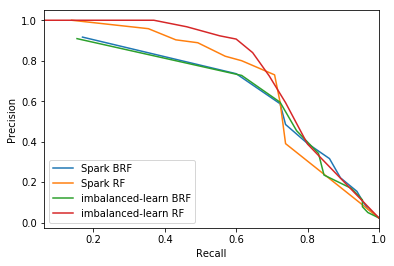
\includegraphics[height=6cm, keepaspectratio]{Figures/test_brf_pr.png}}
\caption{Comparison of implementations: Precision-recall curves}
\label{fig:test-brf-precision-recall}
\end{figure}

Figure~\ref{fig:test-brf-roc} shows the Receiver operating characteristic (ROC) curves obtained with both implementations of the Balanced Random Forest (BRF) and Random Forest (RF) algorithms. Like with the precision-recall curves, we observe BRF implementations perform better with high recall values. 

\begin{figure}[htbp]
\centerline{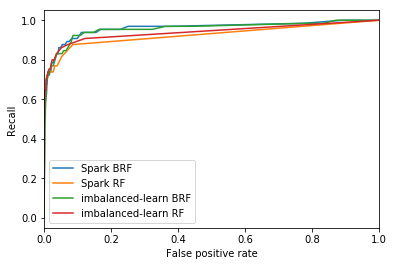
\includegraphics[height=6cm, keepaspectratio]{Figures/test_brf_roc.png}}
\caption{Comparison of implementations: ROC curves}
\label{fig:test-brf-roc}
\end{figure}

\subsection{Vehicle collision prediction}

Results were obtained by training the algorithms on the whole
dataset of positive samples and with a sub-sample of 0.1\% of the 2
billion possible negative examples. This corresponds to a total of 2.3
million examples with a data imbalance reduced to a factor of 17. To
evaluate our models, we used a test set containing the last two years of our
dataset. The model was trained on the 4 previous years and used only data
from these years. For instance, the ``count\_accident" feature contains only
the count of accidents occurring from 2012 to 2016 on the road segment.

Table~\ref{table:summary} presents the results obtained with the classical
Random Forest algorithm (RF), with the Balanced Random Forest algorithm (BRF), and with the XGBoost algorithm without under-sampling (XGB) on the test set.

\begin{table}[htbp]
\caption{Result Summary}
\begin{center}
\begin{tabular}{|l|r|r|r|}
\cline{2-4}
\multicolumn{1}{c|}{} &    BRF &    RF &    XGB \\
\hline
Area under the PR curve &  0.547 &  0.535 &  0.531 \\
Area under the ROC curve &  0.916 &  0.918 &  0.909 \\
\hline
\end{tabular}
\label{table:summary}
\end{center}
\end{table}

Figure~\ref{fig:precision-recall} shows the precision-recall curves of the three models.

\begin{figure}[htbp]
\centerline{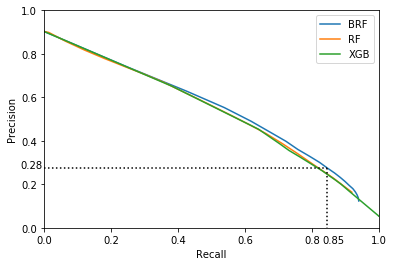
\includegraphics[height=6cm, keepaspectratio]{Figures/pr.png}}
\caption{Vehicle Collision Prediction: Precision-recall curves}
\label{fig:precision-recall}
\end{figure}

Figure~\ref{fig:roc} shows the Receiver operating characteristic (ROC) curves of the three models.

\begin{figure}[htbp]
\centerline{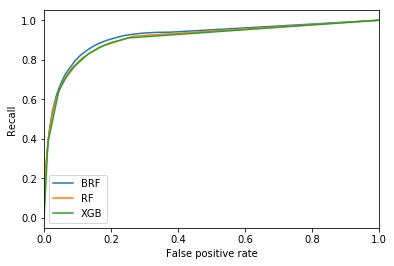
\includegraphics[height=6cm, keepaspectratio]{Figures/roc.png}}
\caption{Vehicle Collision Prediction: ROC curves}
\label{fig:roc}
\end{figure}

As we can see, the Balanced Random Forest model performs slightly better than the other models.
It achieves a recall of $85\%$ with a precision of $28\%$. and a false positive rate (FPR) of $13\%$ on the test set.

% ------------------------
% ------------------------
% ------------------------

\subsection{Vehicle Collision Feature Importance}

With a
feature importance of $67\%$, the number of accidents which occurred on the
road segment during the previous years is clearly the most useful feature, which
is not surprising. Figure~\ref{feature importances} presents the
importance of the other features as reported by the Balanced Random Forest
algorithm. As we can see, the next important feature is the temperature. 
Then, the day of the year, the cosine of the hour of the day, which separates day from night,
and the visibility follow. The solar elevation and the humidity are the next most important features. The remaining features have almost the same importances, except the street type which
is significantly less important.

We believe that the road features like the street length, the street level and the street type have a lower importance because the accident count already provides a lot of information on the dangerousness of a road segment. Surprisingly, the risky weather feature is one of the least important ones. We believe that the temperature, the visibility, the humidity and the atmospheric pressure contains this information in a way that is easier to learn. 

As compared to the count of accidents, the other features seem to have almost no
importance, but the performance of the model decreases significantly if we
remove one of them. 

\begin{figure}[htbp]
\centerline{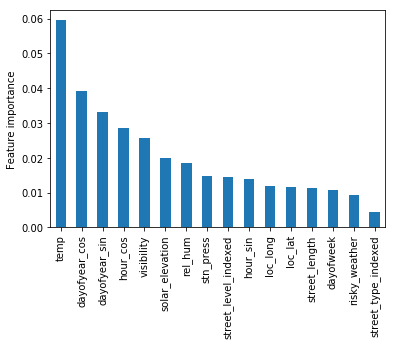
\includegraphics[height=7cm, keepaspectratio]{Figures/brf_fi_nocount.png}}
\caption{Feature importance computed by the Balanced Random Forest excluding the accident count feature.}
\label{feature importances}
\end{figure}

% ------------------------
% ------------------------
% ------------------------

\section{Discussion}
\label{sec:discussion}

With areas under the ROC curve of more than $90\%$, the performances of our models are good.
However, they mostly rely on the count of previous accidents on the road segment. 
This is not an issue for accident prediction, but it does not help to 
understand why these roads are particularly dangerous. We believe that
this feature is even more useful because we do not have information
about the average traffic volume for each road. Therefore, this feature does
not only inform the machine learning algorithm about the dangerousness of a road
segment but also indirectly about the number of vehicles using this road.

\subsection{Test of our implementation of BRF on the mammography dataset}
As expected, we obtained similar results to the imbalanced-learn library with our implementation of the BRF algorithm. Surprinsigly, the BRF algorithm obtained lower areas under the precision-recall curve than the Random Forest algorithm for both implementations. The precision-recall curve explains it, the BRF algorithm had a better precision with high recall values, but a much lower precision with low recall values. For medical diagnosis and road vehicle collision prediction, we usually prefer to have a higher recall with a lower precision, so BRF is more suitable for these usecases. This shows that the measure of the area under the precision-recall curve is not enough to compare the perfomances of a model on given problem, it is necessary to look at the curve. 

\subsection{Comparison of the different models for road vehicle collisions prediction}
For the road vehicle collision prediction, the Balance Random Forest algorithm obtained slightly better results than the classical Random Forest algorithm. However, the gain in prediction performance is small. We believe this is caused by the fact that negative examples are not so different from each other and the information they contain is well captured by a single random sub-sample. Like on the mammography dataset, we observe that the BRF algorithm achieved better performances than Random Forest with high recall values. With lower recall values both Random Forest algorithms had similar performances. The XGBoost algorithm obtained worse results than the two other algorithms. However, it is still interesting because it was much faster to train than Random Forest algorithms. This made the hyper-parameter tuning of the XGBoost algorithm easier and much faster.
\TG{How do you explain the very small added-value of data imbalance techniques?} 

\subsection{Real-world performances of our road vehicle collision prediction model}
\todo{this subsection will be rewritten}
As stated previously, the measure of the accuracy is not a good metric for road accidents prediction. Indeed, since most examples belong to the negative class, the model which obtains the best accuracy is usually the one with the lowest false positive rate. But for rare event prediction, we usually want a model with a high recall even if it implies a higher false positive rate. For these reasons, we decided not to use the measure of the accuracy. Instead we used the precision-recall curve to compare our the performances of our models. However, we should be careful when using the precision measure on a dataset using a sample of the possible negative examples like it is usually the case in accident prediction. Indeed, the precision computed on the test set does not corresponds to the precision we would obtain in production.
If the sample of negative examples is representative of the population
in production, the model will achieve the same false positive rate.
Because we used a sample of the possible negative examples but all the 
positive examples in the test set, there will be more cases of false positive in production for the same number of positives. As a consequence, the precision will be much lower.
For these reasons, we think the best measure to compare the performance of
different studies in accident prediction is the area under the ROC curve.
As opposed to the area under the precision-recall curve, it does not depend on the amount of sub-sampling done on the negative examples. However, to compare two models in the same study both curves are interesting to look at.\TG{mmm, I may not agree with this, let's discuss it.}. 

% ------------------------
% ------------------------
% ------------------------

\subsection{Difference with Other Studies}

Compared to other studies in accident prediction, our study is original by the size of the datasets used and the ``spatial resolution'' of our models' predictions. We call ``spatial resolution'' the precision at which one can estimate the risk of road accident. To the best of our knowledge, some of the related work did either use an important dataset (millions of records in total including hundreds of thousands of positive samples \cite{QChen2016}) or predict at a high resolution (for example making predictions for a given street), but we did not found a study that did both like us. In terms of prediction resolution, some studies worked on only one street \cite{Chang2005} \cite{Chang2005b} \cite{Lin2015} while some others worked on regions (for example 5km by 5km \cite{QChen2016} or 500m by 500m \cite{Yuan2018}). The road accident dataset we used also covers a wider time range than some studies and is about the maximum time range encountered in the related papers we studied: 7 years \cite{Yuan2018} (against 6 years in our case). For example, other studies have worked on accidents occurring during one year \cite{Chang2005} \cite{Chang2005b} \cite{QChen2016} \cite{Lin2015}. In our opinion, the fact that we predict at a higher resolution allow us to get more useful results, but also makes it harder to get good results.

% ------------------------
% ------------------------
% ------------------------

\subsection{Future work}

We believe better performances could be reached by adding more features
from other datasets. For the city of Montreal, we identified two
particularly interesting datasets: a dataset with the location and dates of
construction work on roads, and a dataset with the population density.
In addition, Transport Qu\'ebec gives access to cameras monitoring the main
roads of Montreal. The videos from these cameras could be useful to get an
estimation of the traffic on the island. These datasets might not be as
easily available for other areas, but for Montreal, they could improve 
prediction performances.

The most important feature is the number of accidents which happened during
the previous year. While this feature helps a lot to reach useful prediction
performances, it does not help in understanding the characteristics of a
road segment which makes it dangerous. A human analysis of these
particularly risky road segments could detect patterns that could help to
take measure to reduce the number of accidents in Montreal. This can also
allow to improve our current accident prediction model, if the detected
patterns can be used by fusing other datasets.

\TG{Two comments on the language. (1) Overall it's fine, but many sentences sound 
quite French. In particular, you could reduce your use of ``the": when the noun is indefinite, or when it's unambiguous, just don't use the article.  For instance, ``the" is not needed in ``Section
4 presents how we performed feature engineering, feature
selection and the hyper-parameter tuning", otherwise it puts emphasis on the fact that hyper-parameter tuning is special, which isn't the case. (2) You use ``we believe" a lot and it sometimes reads weird. You can use ``is likely to", or ``may" instead. Since you have time before the submission, and these comments are more relevant when coming from native English speakers, you could go to Concordia's writing assistance and have them read and comment on a page or two of the paper: \url{https://www.concordia.ca/students/success/learning-support/writing-assistance.html}. Again, this is only to improve an already very good writing!}

% ------------------------
% ------------------------
% ------------------------

\section*{Conclusions}

\TG{A conclusion is needed, summarizing the take-home message from the paper:
can your model be used to predict accidents now? at which resolution? how to use it?}
\TG{I didn't read the conclusion as it doesn't look finished.}
In this study we conducted an analysis of road vehicle collisions in the city of Montreal using open data provided by Montreal and the government of Canada. From those datasets we have built road vehicle collision prediction models using tree-based algorithms. By comparing various metrics during the evaluation of our models, we found that there is no perfect measure for the problem under study. 
% ---
First of all, the accuracy is not suited in the case of data imbalance. 
% ---
Second of all, precision and recall are good to reflect the performances, but they are accurate only when the test set has the same class distribution as the real-life class distribution, which can hardly be the case in road accident prediction. 
% ---
Third of all, both ROC and PR curve give different insights and should therefore be used together in future work. The model can predict 85\% of road accident in the area of Montreal at high space resolution and at hourly precision though there is an important amount of false positive. \TG{it would be nice to link this number to an actual results figure.}. We believe our model could be useful to identify the most dangerous time and roads in Montreal. Under the condition that the same kind of datasets are available, we believe that our work can easily be reproduced for other cities. One can freely use our model on Github by loading the model using Spark. Finally, our study shows that open data initiatives to open good quality data are useful to society and allow data science projects of high value by studying important issue for societies like road accidents. 

% ------------------------
% ------------------------
% ------------------------

\section*{Acknowledgment}

The authors would like to acknowledge Compute Canada for providing access to the computation clusters, as well as WestGrid and Calcul Québec, Compute Canada's regional partners for the clusters used.

\bibliographystyle{IEEEtran}
\bibliography{IEEEabrv,Biblio/biblio}

\end{document}
